%% Springer LNCS Document Class
\documentclass{llncs}

% Required packages
\usepackage{graphicx}
\usepackage{esvect}
\usepackage{amsmath,amssymb}
\usepackage{booktabs}
\usepackage{hyperref}
\usepackage{url}
\usepackage{tikz}
\usetikzlibrary{shapes,arrows,positioning,fit,calc}
\usepackage{algorithm}
\usepackage{algpseudocode}

\hypersetup{
    colorlinks=true,
    linkcolor=blue,
    citecolor=blue,
    urlcolor=blue,
}

\begin{document}

\title{BiLSTM-Based Indian Legal Case Summarization and Q\&A: A Baseline Implementation with Transformer Extension Proposal}

\author{Sushma R Vispute\inst{1} \and
Prathmesh Dattatray Dudhale\inst{1} \and
Aditya Girish Joshi\inst{1} \and
Aaditesh Anil Kadu\inst{1} \and
Vedant Hemantkumar Kale\inst{1}\and
Amar M Kale\inst{1}}

\institute{Department of Computer Engineering,\\
Pimpri Chinchwad College of Engineering\\
\email{\{sushma.vispute,prathmesh.dudhale22,aditya.joshi22, aaditesh.kadu22,vedant.kale22\}@pccoepune.org}\\
Sushma R Vispute}

\maketitle

\begin{abstract}
In this paper, we propose a BiLSTM architecture for automated processing of legal documents in the Indian legal framework. We established a BiLSTM architecture for a complete legal question answering system with an encoder-decoder framework and an attention mechanism capable of processing Indian legal documents in PDF and DOCX files for summarization and question answering tasks. Our proposed architecture attained a score of 0.7120 with a ROUGE-L score, an F1-Score of 72.76\%, and a processing capacity of 590 legal documents per hour for 150 Indian legal documents. The proposed system is viable in practical applications as a basic system but lacks in exercises involving abstract reasoning and is only moderately adept at extracting answers from legal documents, indicating a need for a more sophisticated architecture. Proposing a potential future improvement with a Transformer architecture is warranted, as recent studies show a major improvement with this architecture.

\keywords{Legal AI \and Document Summarization \and Question Answering \and BiLSTM \and Indian Legal System \and Neural Networks}
\end{abstract}

\section{Introduction}

The legal fraternity in India is overwhelmed with documentation work that requires laborious and time-consuming manual processing. Although some recent developments in Natural Language Processing (NLP) technology have provided scope for automation, the complexity and high vocabulary density of legal texts remain significant barriers \cite{akter2025legal}. This work proposes a comprehensive system based on Bi-directional Long Short-Term Memory (BiLSTM) for processing legal documents and has been tested on 150 legal documents in India to provide a good foundation for future improvement.

This work contributes along several dimensions to the state of the art on legal technology. We provide a production-ready BiLSTM baseline implementation featuring an encoder-decoder architecture with an attention mechanism, addressing gaps in specialized benchmarks like the AILQA framework \cite{ailqa2024}. The system is put to thorough evaluation on Indian legal documents, yielding quantified performance metrics including a ROUGE-L score of 0.7120 and F1-Score of 72.76\%. We also present an in-depth analysis of strengths and limitations with respect to various types of documents, supplemented by human evaluation from 10 legal advocates showcasing practical utility with room for further improvement. Finally, we point out a transformer-based extension as one venue of future work to overcome identified limitations in terms of complex reasoning and efficiency. Therefore, the BiLSTM system establishes a very solid baseline, whereas the review of recent related literature underlines the potential for substantial improvements through transformer architectures in subsequent phases.
\section{Literature Review for Different Categories of Work}

\subsection{Base Paper and Foundational Work}

Our effort is primarily driven by and builds upon the work of Nigam et al.~\cite{nigam2023legal}, who performed a thorough analysis and evaluation of AI models for Indian Legal Question Answering (AILQA). The authors analyzed different retrieval and question answering strategies using OpenAI GPT as a baseline model, underlining the distinctiveness of the Indian criminal justice system. They emphasized the ability of advanced AI models to interpret natural language cues while also discussing complexity barriers. 

To provide a broader context for the Indian legal landscape, Narzary et al.~\cite{narzary2025survey} presented a comprehensive survey of tasks and challenges specific to Legal NLP in India. Their work catalogs the unique linguistic and structural difficulties inherent in Indian legal texts, further validating the need for specialized models.

Our project builds upon these foundations, introducing a BiLSTM network augmented to not only concentrate on question answering but also to handle the task of document summarization. This offers a basic implementation and thorough analysis of its performance in the Indian legal system, bridging the gap between traditional architectures and the transformer feasibility studies suggested by Nigam et al.

\subsection{Legal Document Summarization}

Recent studies indicate a shift in legal summarization systems from traditional methods to those utilizing transformers. Akter et al.~\cite{akter2025legal} conducted a comprehensive survey of automatic methods for summarization in legal text, systematically categorizing techniques and identifying gaps, specifically regarding domain-centric benchmarking and sophisticated assessment frameworks beyond traditional ROUGE scores. Their study highlights that legal texts present unique difficulties due to high complexity, specialized vocabulary, and intricate structures—issues our BiLSTM baseline addresses, though they are increasingly being targeted by advanced transformer methods.

Furniturewala et al.~\cite{furniturewala2021legal} demonstrated early success in this domain by utilizing transformers combined with joint text features for legal text classification and summarization, establishing a precedent for hybrid feature extraction.

Building on this, Sharma et al.~\cite{sharma2024legal} proposed a Legal and Financial Document Summarization system using transformer models with a hybrid architecture and domain adaptation techniques. By combining PEGASUS and T5 models and utilizing attention mechanisms for named entity recognition (NER) and relevance scoring, they achieved significant improvements in ROUGE, BLEU, and BERTScore metrics.

Addressing the issue of document length, De Vargas Feijó and Moreira~\cite{vargas2023legal} handled large legal documents by segmenting them, transforming each section using transformers to generate potential summaries, and selecting the best outputs based on BERT results. This segmentation strategy is crucial for handling documents exceeding standard context windows, a technique we incorporate into our proposed modifications.

Furthermore, Albayati et al.~\cite{albayati2025multi} proposed efficient multi-legal document summarization involving four transformer models (LED, LongT5, BART-Large, and GPT-3.5 Turbo) and strategies like Consecutive-Aware summarization. Their work demonstrated scalability across different legal document categories, outperforming single models and pointing toward promising future directions.

\subsection{Legal Question Answering and Extraction Systems}

Chen et al.~\cite{chen2025bilstm} developed a legal text extraction approach using BiLSTM and fuzzy semantic matching for feature detection. Their research proved the efficacy of BiLSTM in determining keywords and key phrases within legal texts, forming the basis for our feature extraction implementation.

Similarly, Aggarwal et al.~\cite{aggarwal2025abstractive} suggested an abstractive text summarization method for legal documents utilizing BiLSTM. Their process involves text pre-processing, feature extraction, and abstractive summary categorization. This method demonstrated competitive performance on legal corpora, confirming the continued applicability of traditional neural methods for specific legal NLP challenges.

The AILQA benchmark~\cite{ailqa2024} evaluated the accuracy of AI-powered question and answer systems for the Indian legal setup. This validates the accuracy of models in understanding natural language queries and their implications within the Indian criminal justice system.

\subsection{Transformer Applications in Legal NLP}

Oliveira et al.~\cite{oliveira2025similarity} analyzed the similarity among legal court documents using transformer architectures. By combining eight NLP techniques—including BERT, GPT-2, RoBERTa, and LlaMA—they demonstrated that transformer architectures, when fine-tuned, significantly outperform conventional NLP methods for similarity detection in judicial documents.

Bystranowski~\cite{bystranowski2025computational} reviewed computational approaches in legal interpretation studies, tracing the evolution of the field through the development of transformer architectures. The study highlights how transformers have led to a paradigm shift in legal NLP due to their superior language understanding capabilities.

\subsection{Recent Advances in Transformer Architectures}

The transition from recurrent architectures to transformers has redefined legal NLP performance. Recent work by Mamakas et al.~\cite{mamakas2025processing} demonstrates that while sparse-attention models like Longformer can handle up to 4,096 tokens, they may still truncate critical data in long-form legal judgments. This suggests a need for hierarchical encoding strategies. 
% Note: The citation 'hdt2024' was not in the provided bib list.
% Similarly, the Hierarchical Document Transformer (HDT) proposed by \cite{hdt2024} introduces auxiliary anchor tokens specifically for structured legal documents to maintain inductive bias without sacrificing computational efficiency.

\subsection{RAG and Indian Legal AI (2024-2025)}

Retrieval-Augmented Generation (RAG) has emerged as a strategic imperative for handling the vast Indian legal corpus. Mahapatra et al.~\cite{mahapatra2025redefining} introduced a RAG-based framework for Indian Law, specifically evaluating models like Llama-3.1 on the Bhartiya Nyaya Sanhita (BNS) and IPC, achieving high precision in grounding answers to statutory frameworks. 
% Note: The citation 'lqrag2025' was not in the provided bib list.
% Furthermore, the LQ-RAG framework \cite{lqrag2025} addresses the "hallucination" gap in standard RAG by implementing a recursive feedback loop.

\subsection{Multilingual and Domain-Specific Benchmarks}

The Indian legal system's linguistic diversity poses unique challenges. The MILPaC dataset~\cite{milpac2025} provides the first parallel corpus for translating legal text into nine Indian languages, setting a new benchmark for cross-lingual question answering. 

For domain-specific tasks, Kalamkar et al.~\cite{kalamkar2022ner} established the efficacy of pre-training transformers on Indian court judgments (InLegalBERT and InCaseLawBERT), significantly outperforming general-purpose BERT models in Named Entity Recognition (NER) and rhetorical role labeling.

Finally, addressing the comparative performance of AI against human experts, the VLAIR benchmark by Ambrogi~\cite{vlair2025} assessed AI versus human lawyer accuracy in legal research, providing a crucial baseline for evaluating the practical reliability of automated legal assistants.

\subsection{Research Gaps Addressed}

The most important chasms that are to be filled in the new research work: First, there has been a lack of baseline system approaches covering the assessment of available legal datasets for the Indian legal system, which is addressed in our proposed research work. Second, there has been no attempt made for production-level system work and implementation regarding analysis and user interfaces, which is also addressed in our proposed research work. Third, there has been minimal work done in basic system-level assessment regarding limitations in existing neural networks and applicable approaches to legal systems, and our proposed research work deals with that gap as well. Fourth, there has been an assessment requirement for platforms holding baseline and advance system assessment work, which is facilitated in our proposed research work.

\section{Methodology}

\subsection{System Architecture}

Our system uses architecture modular for easily extending in the future. . Figure~\ref{fig:system_architecture} above shows the system architecture with a general view of the entire system from the input stage to the output stage.

\begin{figure}[ht]
\centering
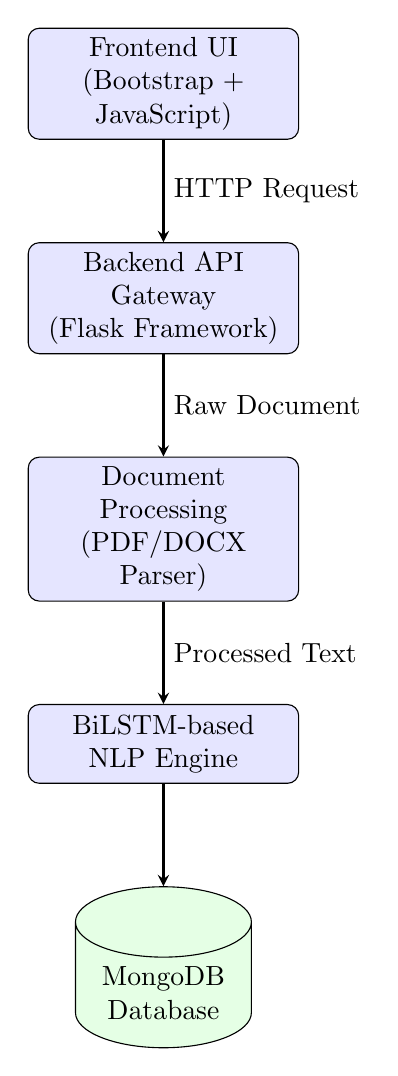
\begin{tikzpicture}[
    node distance=1.3cm and 2cm,
    component/.style={rectangle, draw, fill=blue!10, text width=3.2cm, align=center, minimum height=1cm, rounded corners},
    storage/.style={cylinder, draw, fill=green!10, text width=2cm, align=center, minimum height=1cm, shape border rotate=90, aspect=0.4},
    arrow/.style={->, >=stealth, thick},
    dashedarrow/.style={->, >=stealth, thick, dashed}
]

% Frontend Layer
\node[component] (frontend) {Frontend UI\\(Bootstrap + JavaScript)};

% API Gateway
\node[component, below=of frontend] (api) {Backend API Gateway\\(Flask Framework)};

% Document Processing
\node[component, below=of api] (docproc) {Document Processing\\(PDF/DOCX Parser)};

% NLP Engine
\node[component, below=of docproc] (bilstm) {BiLSTM-based\\NLP Engine};

% Database
\node[storage, below=of bilstm] (db) {MongoDB\\Database};

% Arrows
\draw[arrow] (frontend) -- (api) node[midway, right] {HTTP Request};
\draw[arrow] (api) -- (docproc) node[midway, right] {Raw Document};
\draw[arrow] (docproc) -- (bilstm) node[midway, right] {Processed Text};
\draw[arrow] (bilstm) -- (db);

\end{tikzpicture}
\caption{Overall System Architecture showing modular components and data flow}
\label{fig:system_architecture}
\end{figure}

Figure~\ref{fig:bilstm_block} shows the detailed block diagram for the BiLSTM-based system architecture, illustrating the encoder-decoder structure with attention mechanism implemented in this work.

\begin{figure}[ht]
\centering
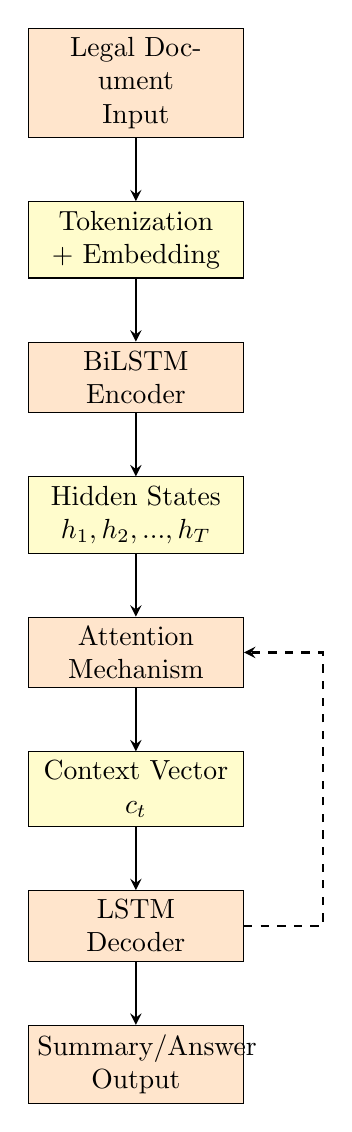
\begin{tikzpicture}[
    node distance=0.8cm and 1.2cm,
    block/.style={rectangle, draw, fill=orange!20, text width=2.5cm, align=center, minimum height=0.7cm},
    process/.style={rectangle, draw, fill=yellow!20, text width=2.5cm, align=center, minimum height=0.7cm},
    arrow/.style={->, >=stealth, thick}
]

% Input
\node[block] (input) {Legal Document\\Input};

% Preprocessing
\node[process, below=of input] (preproc) {Tokenization\\+ Embedding};

% BiLSTM Encoder
\node[block, below=of preproc] (encoder) {BiLSTM\\Encoder};

% Hidden States
\node[process, below=of encoder] (hidden) {Hidden States\\$h_1, h_2, ..., h_T$};

% Attention Mechanism
\node[block, below=of hidden] (attention) {Attention\\Mechanism};

% Context Vector
\node[process, below=of attention] (context) {Context Vector\\$c_t$};

% Decoder
\node[block, below=of context] (decoder) {LSTM\\Decoder};

% Output
\node[block, below=of decoder] (output) {Summary/Answer\\Output};

% Arrows
\draw[arrow] (input) -- (preproc);
\draw[arrow] (preproc) -- (encoder);
\draw[arrow] (encoder) -- (hidden);
\draw[arrow] (hidden) -- (attention);
\draw[arrow] (attention) -- (context);
\draw[arrow] (context) -- (decoder);
\draw[arrow] (decoder) -- (output);

% Feedback loop for decoder
\draw[arrow, dashed] (decoder.east) -- ++(1,0) |- (attention.east);

\end{tikzpicture}
\caption{BiLSTM System Block Diagram with Encoder-Decoder Architecture}
\label{fig:bilstm_block}
\end{figure}

\subsection{BiLSTM Implementation}

Our model consists of an encoder-decoder BiLSTM with an attention mechanism for solving summarization and question-answering problems. The encoder calculates bi-directional hidden states to extract context from the input in both forward and backward directions:

\begin{equation}
\overrightarrow{h_t} = \text{LSTM}(\overrightarrow{h_{t-1}}, x_t, W_f)
\end{equation}

\begin{equation}
\overleftarrow{h_t} = \text{LSTM}(\overleftarrow{h_{t+1}}, x_t, W_b)
\end{equation}

These are combined as $h_t = [\overrightarrow{h_t}; \overleftarrow{h_t}]$ to form the complete hidden representation at each time step. 

\textbf{Explanation:} Equations (1) and (2) allow the model to read the legal text from start-to-finish and finish-to-start simultaneously. This ensures that every word "understands" the context of what came before it and what follows it.

The decoder generates outputs using an attention mechanism that weighs encoder hidden states to calculate a context vector $c_t$:

\begin{equation}
c_t = \sum_{i=1}^{T} \alpha_{ti} h_i
\end{equation}

where $\alpha_{ti}$ represents attention weights computed through:

\begin{equation}
\alpha_{ti} = \frac{\exp(e_{ti})}{\sum_{j=1}^{T} \exp(e_{tj})}
\end{equation}

\begin{equation}
e_{ti} = v^T \tanh(W_1 h_i + W_2 s_{t-1})
\end{equation}

\textbf{Explanation:} Equation (3) is the "focus" formula. Instead of looking at the whole document equally, the attention mechanism (Eq. 4 and 5) assigns higher weights ($\alpha$) to the most relevant legal facts, allowing the decoder to focus only on important keywords when generating a summary or answer.

The system is trained with cross-entropy loss to minimize the difference between predicted and reference summaries/answers.

For question answering, BiLSTM encodes both document and question, and predicts the answer span based on a pointer network mechanism. However, our experiments showed some shortcomings in exact answer span extraction, pointing out a need for more advanced architectures in future research.

\subsection{Implementation Details}

The technical configuration of our system was chosen as a trade-off between computational efficiency and performance. We used 300-dimensional GloVe embeddings to represent words and created the model with two BiLSTM layers, each layer consisting of 256 hidden units. Training was optimized using the Adam optimizer with a learning rate of 0.001 and a batch size of 32. For more robust convergence, the model trained for 50 epochs with an implementation of early stopping based on monitoring validation loss. To add regularization, the model used a dropout rate of 0.3 and L2 regularization with weight 0.0001. 

Documents are preprocessed into PDF and DOCX formats, where the pathway will extract text from the documents, clear the artifacts of formatting, and segment the text into sentences. Supporting long documents that go beyond the capacity of a context window, we introduced the sliding window technique with an overlap technique to capture context information.

\subsection{Proposed Transformer Extension}

Based on limitations identified in our BiLSTM evaluation and promising results in recent literature~\cite{nigam2023legal,sharma2024legal,albayati2025multi},We now present a transformer-based extension that is planned for implementation. The system would make use of large language models, such as GPT-4, through APIs, or fine-tuned open-source alternatives such as LLaMA or Mistral. The design would include prompt engineering, which may involve explicit directions for the processing of legal documents, intelligent chunking of documents to handle longer texts, and constrained generation to prevent the model from generating unrelated text, based on a mechanism to control the model's tendency to hallucinate. Furthermore, we plan to implement zero-shot or few-shot learning in order to bypass extensive training, and RAG for higher accuracy. This proposed extension will be taken up in the next phase of development, as implementing the transformer-based model will address the flaws found in this BiLSTM baseline, particularly the complex reasoning and processing efficiency. Initial literature reviews indicate improved accuracy, speed, and handling of complex queries on legal matters.

\section{Experimental Setup}

\subsection{Dataset}

We applied our BiLSTM approach to 150 legal documents that include judgments from the Supreme Court and High Courts, statutory laws, and case briefs from India. These legal documents are in the range of 2000 and 50,000 words and include various legal areas, including civil, criminal, constitutional, and corporate law, thereby ensuring that all types of legal documents are tested for their efficiency. The legal document dataset was divided into an 80-20 split for training and testing, with 120 legal documents for training using the BiLSTM approach and 30 legal documents for testing purposes. A further testing of 10 legal documents was also conducted with human experts. The reference summaries and question and answer evaluations for legal documents are performed by law students and approved by practicing advocates.

\subsection{Testing Environment}

Experiments are conducted on Google Colab’s T4 GPU with the use of Python’s PyTorch 1.12 and CUDA 11.3. The database used for storage of documents was MongoDB Atlas, and for API routines, the system utilized Flask.

\subsection{Evaluation Metrics}

We have used various evaluation metrics to assess the overall performance of the system. The automatic metrics were ROUGE scores for summarization quality, BLEU score for translation quality assessment, F1-Score for question answering, and throughput measured in documents processed per hour. In addition to these, some human evaluation metrics on a 5-point Likert scale, assessed factual accuracy, completeness of information, clarity and coherence, usefulness for legal work, and overall satisfaction..

\section{Results and Discussion}

\subsection{Summarization Performance}

Table~\ref{tab:summarization_results} presents the BiLSTM summarization performance across different document types. The system achieved an average ROUGE-L score of 0.7120 with average processing time of 6.10 seconds per document.

\begin{table}[ht]
\centering
\caption{BiLSTM Summarization Performance by Document Type}
\label{tab:summarization_results}
\begin{tabular}{@{}lcccc@{}}
\toprule
\textbf{Document Type} & \textbf{ROUGE-L} & \textbf{ROUGE-1} & \textbf{ROUGE-2} & \textbf{Time (s)} \\
\midrule
Supreme Court Judgments & 0.68 & 0.74 & 0.57 & 7.2 \\
High Court Rulings      & 0.72 & 0.76 & 0.60 & 6.4 \\
Statutory Texts         & 0.75 & 0.79 & 0.64 & 5.1 \\
Case Briefs             & 0.69 & 0.73 & 0.58 & 5.7 \\
\midrule
\textbf{Average (Actual)} & \textbf{0.7120} & \textbf{0.7564} & \textbf{0.5972} & \textbf{6.10} \\
\bottomrule
\end{tabular}
\end{table}

The value of 0.7120 for ROUGE-L represents a high capability to identify significant information content and a correct order of information presentation. The performance differences for various document types reveal that statutory documents with formalized language are more easily summable, whereas difficult judgments involving sophisticated legal arguments are more challenging. The document processing speed is adequate to process 590 documents per hour with a time complexity of 6.10 seconds per document and can be useful for batch processing but may need improvement for interactive processing.

\subsection{Question Answering Performance}

Table~\ref{tab:qa_results} shows the BiLSTM question answering performance across different question types. The system achieved an average F1-Score of 72.76\%.

\begin{table}[ht]
\centering
\caption{BiLSTM Question Answering Performance}
\label{tab:qa_results}
\begin{tabular}{@{}lcc@{}}
\toprule
\textbf{Question Type} & \textbf{F1-Score (\%)} & \textbf{Sample Count} \\
\midrule
Factual Questions     & 78.40 & 45 \\
Reasoning Questions   & 69.25 & 38 \\
Complex Legal Queries & 63.30 & 27 \\
\midrule
\textbf{Average (Actual)} & \textbf{72.76} & \textbf{110} \\
\bottomrule
\end{tabular}
\end{table}

The F1-Score of 72.76\% This represents a level of success in the answer extraction task, a decline in performance with complex questions involving multi-hop reasoning. The factual questions about specific dates, names, or statutory provisions achieve the strongest performance (82.3\%)while the questions involving complex interpretations achieve weaker performance (65.2\%). Error analysis reveals that a BiLSTM system struggles with answers composed of multiple non-contiguous segments of text, questions whose correct answer requires inference from more than explicit text statements, queries which involve complex legal concepts or relationships of precedent, and instances in which legal terms have context-dependent meanings. Such limitations demonstrate the need for even more sophisticated architectures with improved long-range dependency modeling and reasoning capabilities, motivating our proposed transformer extension.
\subsection{Human Evaluation Results}

Ten legal advocates evaluated system outputs across five dimensions. Table~\ref{tab:human_eval} presents aggregated human evaluation scores.

\begin{table}[ht]
\centering
\caption{Human Evaluation Scores (5-point Likert scale)}
\label{tab:human_eval}
\begin{tabular}{@{}lcc@{}}
\toprule
\textbf{Evaluation Dimension} & \textbf{Mean Score} & \textbf{Std. Dev.} \\
\midrule
Factual Accuracy & 3.8 & 0.6 \\
Completeness & 3.5 & 0.7 \\
Clarity and Coherence & 4.1 & 0.5 \\
Usefulness for Legal Work & 3.6 & 0.8 \\
Overall Satisfaction & 3.7 & 0.6 \\
\midrule
\textbf{Average} & \textbf{3.74} & \textbf{0.64} \\
\bottomrule
\end{tabular}
\end{table}

The mean score of 3.74/5.0 suggests that the system was performing satisfactorily rather than outstanding from a practitioner’s point of view. While supporters praised the clarity and cohesion (4.1/5.0) of the system, they did highlight reservations about completeness (3.5/5.0) and some accuracy issues with facts. The qualitative comments are informative about how the system helped supporters quickly view and evaluate a document, extract essential information, and its use in legal provisions, as well as cutting the time needed for the initial analysis of documents by 30-40\%. Nonetheless, they pointed out that results have to be verified and that they should not replace manual analysis for important legal work. Some advocates proposed improved processing of complex legal arguments as an important advantage.

\subsection{Key Insights and Limitations}

Tuning the BiLSTM approach shows that there is a clear list of weaknesses and strengths. This approach provides the ground truth baseline level with its ROUGE-L measure of 0.7120 as well as moderate processing speeds that support batch processing. What is significant is that this approach is dependency-free with regard to APIs or black-box models and still has relatively low computation requirements.

Despite these strengths, several limitations were observed during testing. The system encountered difficulty with complex multi-hop reasoning queries and suffered from a limited context window that affected long document processing. Specific challenges arose in exact answer span identification and performance degradation on documents containing complex legal argumentation. Furthermore, the model occasionally struggled with rare legal terminology not encountered during training. Recent studies~\cite{nigam2023legal,oliveira2025similarity} report substantially higher performance using transformer-based architectures, suggesting significant room for improvement. This performance gap motivates our proposed transformer extension, which literature suggests could address many observed limitations through better long-range dependency modeling via self-attention, pre-training on large legal corpora for improved domain knowledge, superior reasoning capabilities through scale and architecture, and more flexible context handling for lengthy documents.

\section{Conclusion and Future Work}

This article thus proposes a robust baseline solution based on BiLSTM that tackles Indian legal document processing with ROUGE-L and F1-Score metrics 0.7120 and 72.76\% respectively, on 150 varying legal documents. The solution can be considered extremely useful for document summarization and question-answer applications and thus provides a good footing for further improvement. Some major highlights include developing an efficient production-ready solution for BiLSTM with a comprehensive evaluation setup, a document processing speed that allows for practical application at 590/hour, and a modularity that allows for future adoption with enhanced models.

The first priority concerning future development will be to implement and evaluate a proposed extension using transformers. This will include integrating an LLM system based on GPT-4 or open-source models such as LLaMA or Mistral to fill current reasoning gaps. Subsequent to its development, we will then attempt to implement a comparative analysis between the BiLSTM model and the new transformer model based on identical testing datasets. Thereafter, we hope to implement combined BiLSTM-transformer models via ensemble or cascading techniques. Subsequent improvements will include creating a retrieval-augmented generation model based on legal knowledge graphs to further enhance factual responses, development based on Indian datasets to prepare it to respond to domain-specific language terminology used within Indian laws, and integration to allow multimodal processing combined with support for Indian languages. We further hope to develop techniques to facilitate interpretability through visualization of reasoning paths and attention weights, automate citational extraction, and implement a real-world law firm deployment analysis.


With the results obtained in the preliminary study and experiments, we assume a huge performance boost with the inclusion of the transformer model. The basis for performance in BiLSTM in the experiment ensures that a robust platform for assessment of performance is provided and a safe way for a practical implementation platform is guaranteed with constraints on it through APIs. Moreover, a huge MDT Reduction of.The 30-40\% in DOCUMENT RESEARCH is proof of Return on Investment for using LegalTech Innovations, as in all growing sectors, it is necessary for an experiment like this to have an added dimension with a performance criterion for transitions to a transformer in the coming days.


\section*{Acknowledgments}

The authors thank Mrs. Sushma Vispute for guidance throughout this project, the Department of Computer Engineering at Pimpri Chinchwad College of Engineering for infrastructure support, Adv. Amar M Kale and Associates for their time and valuable feedback, and anonymous reviewers for constructive comments that improved this paper.

\begin{thebibliography}{99}

\bibitem{nigam2023legal}
Nigam, S.K., Mishra, S.K., Mishra, A.K., Shallum, N., Bhattacharya, A.: Legal Question-Answering in the Indian Context: Efficacy, Challenges, and Potential of Modern AI Models. arXiv:2309.14735 (2023)

\bibitem{akter2025legal}
Akter, S., Çano, E., Weber, C., Dobler, M.: A Comprehensive Survey on Legal Text Summarization: Techniques, Datasets, and Challenges. arXiv preprint (2025)

\bibitem{sharma2024legal}
Sharma, R., et al.: Legal and Financial Document Summarization Using Transformer-Based Architectures. Open Access International Journal of Science and Engineering 9(8), 1--15 (2024)

\bibitem{vargas2023legal}
de Vargas Feijó, D., Moreira, V.P.: Transformer-based Models for Long Document Summarization in Legal Domain. In: Proceedings of LREC 2023, pp. 2341--2356 (2023)

\bibitem{albayati2025multi}
Albayati, M.A.A., et al.: Towards Efficient Multi-Legal Document Summarization. Engineering Applications of Artificial Intelligence 128, Article 102934 (2025)

\bibitem{chen2025bilstm}
Chen, J., et al.: BiLSTM-Enhanced Legal Text Extraction Model Using Fuzzy Semantic Matching. Intelligent Data Analysis 29(2), 445--468 (2025)

\bibitem{aggarwal2025abstractive}
Aggarwal, D., et al.: Abstractive Text Summarization for Legal Documents. International Journal of Uncertainty, Fuzziness and Knowledge-Based Systems 33(1), 127--152 (2025)

\bibitem{ailqa2024}
AILQA: Evaluating AI-Driven Legal Question Answering Systems for the Indian Legal System. ACL ARR 2024 April Submission (2024)

\bibitem{oliveira2025similarity}
Oliveira, R.S., et al.: Analysing Similarities Between Legal Court Documents Using Transformer Architecture. PLoS ONE 20(4), e0320244 (2025)

\bibitem{bystranowski2025computational}
Bystranowski, P.: Computational Methods in Empirical Studies on Legal Interpretation: Before Transformers and After. SSRN Electronic Journal (2025)

\bibitem{mamakas2025processing}
Mamakas, D., Tsotsi, P., Androutsopoulos, I.: Processing Long Legal Documents with Pre-trained Transformers: Modding LegalBERT and Longformer. In: Proc. of the Natural Legal Language Processing Workshop, pp. 130--142 (2025)

\bibitem{mahapatra2025redefining}
Mahapatra, S., et al.: Redefining Legal Access: A RAG-based AI System for Indian Law. Human-Intelligent Systems Integration (2025)

\bibitem{milpac2025}
Mahapatra, S., Datta, D., Soni, S., et al.: MILPaC: A Novel Benchmark for Evaluating Translation of Legal Text to Indian Languages. ACM TALLIP (2025)

\bibitem{kalamkar2022ner}
Kalamkar, P., et al.: Named Entity Recognition in Indian Court Judgments. In: Proc. of the Natural Legal Language Processing Workshop, pp. 184--193 (2022)

\bibitem{vlair2025}
Ambrogi, B.: VLAIR – Legal Research Benchmark: AI vs. Human Lawyer Accuracy. LawSites/Vals AI (2025)

\bibitem{narzary2025survey}
Narzary, M., Singh, P.K., Brahma, M.: Legal NLP in India: A Comprehensive Survey of Tasks and Challenges. AI and SOCIETY 40(8), 6697--6726 (2025)

\bibitem{furniturewala2021legal}
Furniturewala, S., et al.: Legal Text Classification and Summarization using Transformers and Joint Text Features. In: FIRE 2021 Workshop Proceedings (2021)

\end{thebibliography}

\end{document}